%% THE PAPER. Write here: sections/*.tex. Grey [notes] say what goes where (from the 29 Oct call with Jerome) and
%% disappear with \shownotesfalse below. The reference draft is draft.tex / draft.pdf; nothing here depends on it.
\documentclass{article}
%% Shared by main.tex (the paper you write) and draft.tex (the reference draft).
%% Format: the ICML 2026 kit, two columns, Times text and Computer Modern math. Page geometry, fonts and spacing
%% come from the kit and are never changed here. The kit is the provisional choice until the venue is decided:
%% for a journal (e.g. PRX Intelligence, revtex two-column), only this file and the \twocolumn[...] block in the
%% two main files change.

\usepackage{microtype}
\usepackage{graphicx}
\usepackage{booktabs}
\usepackage{xcolor}
\usepackage{hyperref}
\usepackage{tikz}
\usetikzlibrary{arrows.meta,calc,positioning}
\newcommand{\theHalgorithm}{\arabic{algorithm}}

% preprint: author names shown, footer "Preprint. <date>" (arXiv first, venue later).
% Anonymous submission: \usepackage{icml2026}.  Camera-ready: \usepackage[accepted]{icml2026}.
\usepackage[preprint]{icml2026}

\usepackage{amsmath}
\usepackage{amssymb}
\usepackage{mathtools}
\usepackage[capitalize,noabbrev]{cleveref}

\graphicspath{{figures/}}

%% ---------------------------------------------------------------- figures
%% Every plot is drawn at its printed size: 3.25 in for one column, 6.75 in for the full width (figure*).
%% Include them WITHOUT a width, so that the axis labels stay at the body's 10 pt:
%%     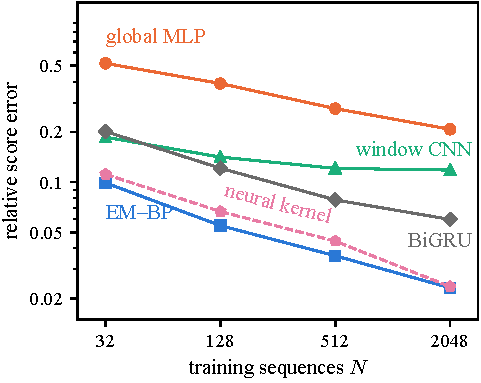
\includegraphics{fig_value_of_structure}
%% The plots and their style (box on all four sides, no grid, minor ticks, log scales, markers for measurements and
%% lines for closed forms) are made by tools/paper_figs/make_paper_figures.py in the research repository; see README.md.
%% The two diagrams are TikZ, \input from figures/*.tikz, so they use the body font and can be edited here.

%% ---------------------------------------------------------------- notation
\newcommand{\E}{\mathbb{E}}
\newcommand{\Normal}{\mathcal{N}}
\newcommand{\Kt}{K_\theta}
\newcommand{\dd}{\mathrm{d}}
\newcommand{\Dt}{\Delta_t}
\newcommand{\Ng}{N_g}

%% ---------------------------------------------------------------- writing aids
%% \note{...}    grey guidance text: what goes here, what Jerome asked for. Hide them all with \shownotesfalse.
%% \pending{...} a result that is not in yet (a run still on the cluster). Shown in orange so none is forgotten.
\newif\ifshownotes \shownotestrue
\definecolor{notegrey}{gray}{0.45}
\definecolor{pendingorange}{HTML}{C0501F}
\newcommand{\note}[1]{\ifshownotes{\color{notegrey}\itshape [#1]}\fi}
\newcommand{\pending}[1]{{\color{pendingorange}[pending: #1]}}

% \shownotesfalse

\icmltitlerunning{Learning Scores for Markov Sequences in Generative Diffusion}

\begin{document}

\twocolumn[
\icmltitle{Title}

\begin{icmlauthorlist}
  \icmlauthor{Giovanni Mantovani}{boc}
  \icmlauthor{J\'er\^ome Garnier-Brun}{boc}
  \icmlauthor{Marc M\'ezard}{boc}
\end{icmlauthorlist}
\icmlaffiliation{boc}{Department of Computing Sciences, Bocconi University, Milan, Italy}
\icmlcorrespondingauthor{Giovanni Mantovani}{giovanni-mantovani@studbocconi.it}
\icmlkeywords{diffusion models, belief propagation, expectation maximisation, Markov chains}
\vskip 0.3in
]

\printAffiliationsAndNotice{}

\begin{abstract}
\note{Five or six sentences, in the order of the paper: (1) a diffusion model needs a denoiser; Markov sequences
(time series, 1-D fields) fix its form. (2) Gaussian chain: diffusion breaks locality, the score is not local.
(3) Chain + noise = tree, so BP gives the exact score from the kernel. (4) Learn the kernel by EM with BP as E-step,
from noisy data. (5) Laplace chain: learned kernel vs networks (best network 2.1--2.8$\times$, MLP 5.8--9.9$\times$);
how it degrades off-Markov. (6) Allen--Cahn: the family matters; parameters recovered.}

Diffusion models learn to denoise a process at every time step $t$. To accomplish this, the score is the fundamental object that is needed, which is an affine function of the posterior mean. We ask how to do this for Markov sequences. Starting with the Gaussian case, where the score is linear and depends on the precision matrix, we see how noise quickly erases the Markov structure. In the Laplace case, the score does not have a closed form anymore, and we notice that the factor graph is a tree; hence, we can get the exact score via Belief Propagation. Messages are probability densities; we then use a grid to discretize them, and the discretization error is tested with the Gaussian closed form. Subsequently, we then want to estimate the kernel, either with Expectation Maximisation over latent variables or Maximum Likelihood over the clean sequence. Moreover, we run experiments on a suitable physical model, such as the stochastic Allen-Cahn field, comparing many kernels from different parametric families with more flexible neural kernels. Finally, we show that in Markov sequences, it can be beneficial to train small neural kernels and recover the score through BP rather than using neural networks to denoise the score directly.

\end{abstract}

\section{Introduction}
\label{sec:intro}

\note{About one column. J\'er\^ome (47:03--48:37): less is more, little background, do not explain diffusion, ``we
want a denoiser''; \textbackslash cite\{\} placeholders are fine, he will help with the literature.}

\note{Framing (12:01, 33:47): data with a direction, temporal causality, a Markov chain; in physics most processes are
local. The question: what does a denoiser gain from knowing the data are Markov, and how should it use it? For an ML
venue: why this question matters for this type of structure. For a physics journal: a protocol for dynamical systems
with this structure.}

\note{The three steps, one paragraph each or one paragraph in all: the score is not local (Sec.~3); the posterior is a
tree, BP is exact (Sec.~4); learning = learning the kernel by EM, no backpropagation through BP (Sec.~5). Then the
experiments: Laplace chain vs networks, off-Markov; Allen--Cahn (Sec.~6).}

Diffusion models are inspired by nonequilibrium thermodynamics (Noneq diff models) techinques and are state-of-the-art generative models widely used to generate pictures (DALL-E 3, OpenAI), videos (Google Veo), 3D protein structures (AlphaFold3), and many other applications. These models reverse an SDE (DSM with SDEs, DDPM) using the score $s_t(\mathbf{x}_t)
=
\nabla_{\mathbf{x}_t}
\log p_t(\mathbf{x}_t).$ which can be rewritten as a posterior mean estimation problem. Notable work has been done on the understanding of the models with the identification of dynamical regimes (Mezard Biroli), explanation on why generalization emerges (Mezard Biroli Bonnaire), and biased generalization (Garnier-Brun Mezard). 
Here we work with Markov sequences, and we want to understand what a denoiser gains from knowing the data is Markov and how we can exploit this property.
We start from the simple Gaussian case where the score has a linear closed form and we study the precision matrix that characterizes it. Then, the most controlled case where the score is non linear is the Laplace case and we can compute exact scores using message passing. Finally, we learn the kernel and we run experiments on the stochastic Allen-Cahn physical model.

The main contributions are:

- For any first order Markov chain, we can recover the exact score using Belief Propagation

- In Markov sequences where you do not know the kernel, you can learn it through Expectation Maximization if you see just noisy sequences or Maximum Likelihood if you have access to the clean sequences. You can even use a small neural network and recover the score with BP, which more accurate and more efficient, in our experiments, compared to denoising score matching. 

- Estimation of the discretization error using a grid with the Gaussian reference

- Characterization of the Gaussian case and Laplace case and generalization to any distribution.



\section{Setting}
\label{sec:setting}

\note{Half a column. Only what the rest needs: the chain $p_0(a)=\mu(a_1)\prod_kK(a_{k+1}\mid a_k)$, same kernel at
every site (J\'er\^ome asked, 14:26: say a site-dependent kernel also works); OU noise
$x_k=e^{-t}a_k+\sqrt{\Delta_t}\,\xi_k$; Tweedie, score $=(e^{-t}\E[a\mid x]-x)/\Delta_t$; the Gaussian and the Laplace
chain with the same covariance ($\alpha=0.85$, $L=32$); the relative score error pooled over twelve levels
$t\in[0.05,3]$.}

\begin{equation}
  p_0(a)=\mu(a_1)\prod_{k=1}^{L-1}K(a_{k+1}\mid a_k)
  \label{eq:chain}
\end{equation}

\begin{equation}
  S_t(x)_k=\frac{e^{-t}\,\E[a_k\mid x]-x_k}{\Delta_t}
  \label{eq:tweedie}
\end{equation}

\section{The Gaussian chain: diffusion breaks locality}
\label{sec:gaussian}

\begin{figure*}[t]
  \centering
  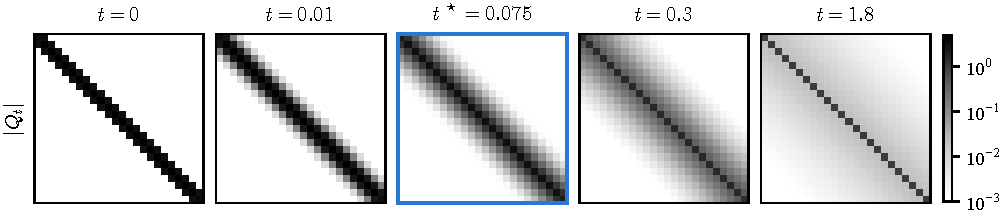
\includegraphics{fig_locality}
  \caption{\note{$|Q_t|$ of the Gaussian chain ($\alpha=0.85$, $L=24$) at $t=0$, $0.01$, $t^\star=0.075$, $0.3$,
  $1.8$: tridiagonal at $t=0$, densest at $t^\star$ (framed), diagonal at large $t$. Slide 5.}}
  \label{fig:locality}
\end{figure*}

\note{J\'er\^ome (12:01, 33:47): the denoiser is tridiagonal only for a while; diffusion breaks locality; so locality
cannot be had by stupidly fitting a tridiagonal matrix. Score $=-Q_tx$, $Q_t=(e^{-2t}\Sigma_0+\Delta_tI)^{-1}$.}

\note{Numbers: $t^\star=0.0753$ (generator printout). Best denoiser restricted to a window of radius $r$, Gaussian
chain, infinite data: relative score error $0.20$ ($r=1$), $0.089$ ($r=2$), $0.029$ ($r=4$), $0.0066$ ($r=8$)
--- thesis \texttt{fig\_ch10.windowed\_oracle}.}

\note{End: the posterior is still a chain; for the Gaussian chain inference on it is the Kalman smoother.}

\section{A noisy Markov chain is a tree}
\label{sec:tree}

\begin{figure}[t]
  \centering
  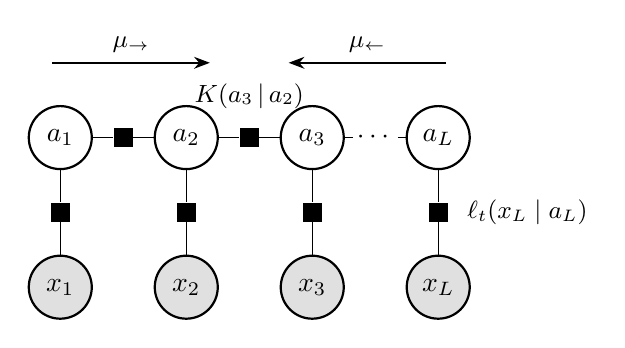
\begin{tikzpicture}[
    var/.style={circle,draw,thick,minimum size=8mm,inner sep=0pt},
    obs/.style={circle,draw,thick,fill=black!12,minimum size=8mm,inner sep=0pt},
    fac/.style={rectangle,fill=black,minimum size=2.4mm,inner sep=0pt},
    lab/.style={font=\small}]
  \foreach \i/\n in {0/1,1/2,2/3,3/L} {
    \node[var] (a\i) at (1.6*\i,0) {$a_{\n}$};
    \node[fac] (o\i) at (1.6*\i,-0.95) {};
    \node[obs] (x\i) at (1.6*\i,-1.9) {$x_{\n}$};
    \draw (a\i) -- (o\i) -- (x\i);
  }
  \foreach \i/\j in {0/1,1/2} {
    \node[fac] (k\i) at ($(a\i)!0.5!(a\j)$) {};
    \draw (a\i) -- (k\i) -- (a\j);
  }
  \draw (a2) -- ($(a2)!0.32!(a3)$);
  \node at ($(a2)!0.5!(a3)$) {$\cdots$};
  \draw ($(a2)!0.68!(a3)$) -- (a3);
  \node[lab,above=1.2mm of k1] {$K(a_3\,|\,a_2)$};
  \node[lab,right=1.2mm of o3] {$\ell_t(x_L\mid a_L)$};
  \draw[-{Stealth[length=2mm]},thick] ($(a0)+(-0.1,0.95)$) -- node[above,lab]{$\mu_{\to}$} ($(a1)+(0.3,0.95)$);
  \draw[-{Stealth[length=2mm]},thick] ($(a3)+(0.1,0.95)$) -- node[above,lab]{$\mu_{\leftarrow}$} ($(a2)+(-0.3,0.95)$);
\end{tikzpicture}

  \caption{\note{Factor graph of $p(a\mid x)$: kernel factors between neighbours, noise factors $\ell_t$ at each
  site; no loop, so BP is exact. Messages $\mu_\to$, $\mu_\leftarrow$. Slide 7.}}
  \label{fig:factor-graph}
\end{figure}

\note{J\'er\^ome (49:16): put the factor graph in, it shows at a glance that the model is a tree, which is not obvious
even to statistical physicists. BP at the level of his hierarchical-filtering paper \S2.4, ``maybe a bit more
detailed'' (48:37); BP on the grid is ``a bit detailed'' (50:20), so the grid recursions go to Appendix~A. Solve the
exactly known case here (12:01).}

\note{BP: forward and backward messages, marginal $\propto\mu_\to\mu_\leftarrow$, mean $\to$ score by
\cref{eq:tweedie}; any kernel, any $t$. On a grid: $N_g=401$ points, matrix--vector products, $O(LN_g^2)$.
Grid exactness: round-off on the Gaussian chain for $t\geq0.05$ (Appendix~A); about $10^{-5}$ on the Laplace chain.}

\begin{figure*}[t]
  \centering
  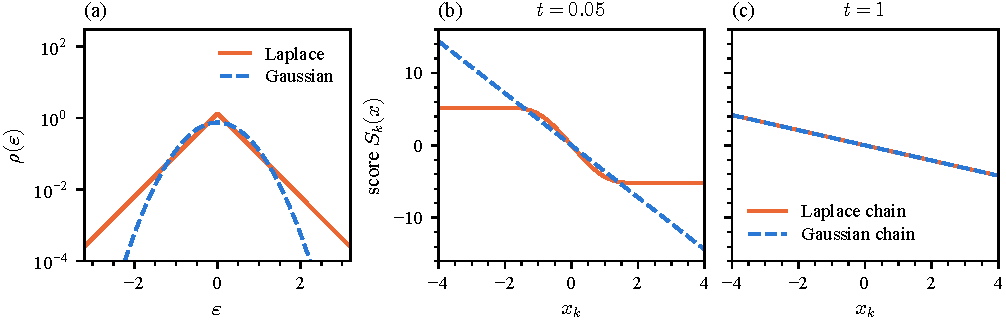
\includegraphics{fig_laplace}
  \caption{\note{(a) Laplace vs Gaussian innovation, same variance. (b, c) Score of the middle site against $x_k$ at
  $t=0.05$ and $t=1$: saturates at small noise, linear at large noise. Slide 6.}}
  \label{fig:laplace}
\end{figure*}

\begin{figure}[t]
  \centering
  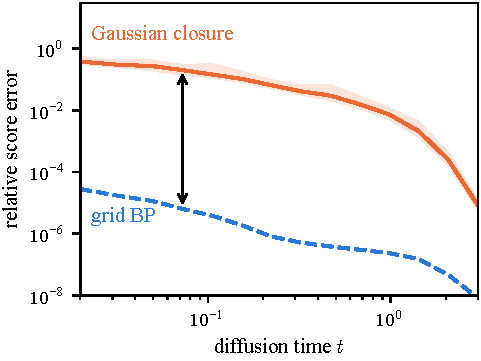
\includegraphics{fig_closure}
  \caption{\note{Laplace chain, true kernel: the best linear denoiser (Gaussian closure / Kalman) against grid BP's
  own error. Slide 8.}}
  \label{fig:closure}
\end{figure}

\note{Numbers: closure error median $0.27$ at $t=0.05$ ($0.38$ at $t=0.02$, $8\times10^{-6}$ at $t=3$) against grid
error $1.1\times10^{-5}$ --- thesis \texttt{tools/data/ch07\_metrics.csv}.}

\section{Messages are probability densities}
\label{sec:grid}

Unlike discrete-state models, here each latent variable
$a_k\in\mathbb R$. Consequently, a belief-propagation message
is a non-negative function of a continuous variable, rather
than a finite-dimensional vector. The message updates therefore
involve integrals over $\mathbb R$, which cannot in general be
evaluated in closed form for a non-Gaussian transition kernel.

We approximate these integrals numerically by discretising the
state space. We introduce a uniform grid
\begin{equation}
    g_i=-A+ih,\qquad i=0,\ldots,N_g-1,
    \qquad h=\frac{2A}{N_g-1},
\end{equation}
on $[-A,A]$, together with trapezoidal quadrature weights
$w_i$. The transition kernel and observation likelihood are
then evaluated on the grid:
\begin{equation}
    K_{ij}=K(g_i\mid g_j),
    \qquad
    (\ell_k)_i=\ell_t(x_k\mid g_i).
\end{equation}
Each integral in the forward and backward recursions becomes
a weighted matrix--vector product. In particular, the
unnormalised updates are
\begin{align}
    f_{k+1}
    &\propto
    \ell_k\odot K(w\odot f_k),\\
    b_k
    &\propto
    K^\top(w\odot\ell_{k+1}\odot b_{k+1}),
\end{align}
where $\odot$ denotes elementwise multiplication and
$w=(w_0,\ldots,w_{N_g-1})^\top$.
The messages are normalised after each update to ensure
numerical stability. The posterior mean is approximated by
\begin{equation}
    \widehat m_k
    =
    \frac{\sum_i w_i g_i(f_k)_i(b_k)_i}
         {\sum_i w_i(f_k)_i(b_k)_i},
\end{equation}
and substituted into the Tweedie identity to obtain the score.

The resulting computational cost is
$O(LN_g^2)$, with $N_g$ grid points and sequence length $L$.
Although this introduces a discretization error, its
accuracy can be controlled by refining the grid and enlarging
the integration domain, and against the Gaussian reference.

\paragraph{Why not a Gaussian approximation?}
A natural alternative would be to approximate each message
by a Gaussian distribution, retaining only its mean and
variance. This is exact for the Gaussian chain: Gaussian
likelihoods and transition kernels are closed under the
multiplication and marginalisation operations of belief
propagation. It is not exact for the Laplace chain, however.
A Gaussian closure discards the non-Gaussian features of the
messages and effectively recovers the score of the
covariance-matched Gaussian model.

This distinction matters most at low noise, where the
Laplace-chain score exhibits a non-linear, saturating
dependence on the observations. As shown in
Fig.~\ref{fig:grid-vs-gaussian}, the Gaussian approximation
can therefore incur substantial score error, whereas grid
belief propagation closely tracks the reference solution.

This should also be distinguished from approximate message
passing (AMP) and Thouless--Anderson--Palmer (TAP) methods.
Those methods are motivated by dense, high-dimensional
systems, where many weak interactions justify approximate
Gaussian message updates, often with an Onsager correction.
Our factor graph is instead a finite-degree chain and a tree:
ordinary belief propagation is already exact at the
continuous level. We therefore discretise the messages
rather than introduce a Gaussian approximation.
\section{Learning the kernel: the Laplace chain}
\label{sec:laplace}

\note{The largest section (33:47): ``the heart of the proposal is EM on Markov chains'' (29:29). The whole
comparison with a network that has locality (CNN) and one that has none (MLP), then breaking Markovianity, in the main
text.}

\subsection{Expectation--maximisation through BP}
\label{sec:em}

\begin{figure}[t]
  \centering
  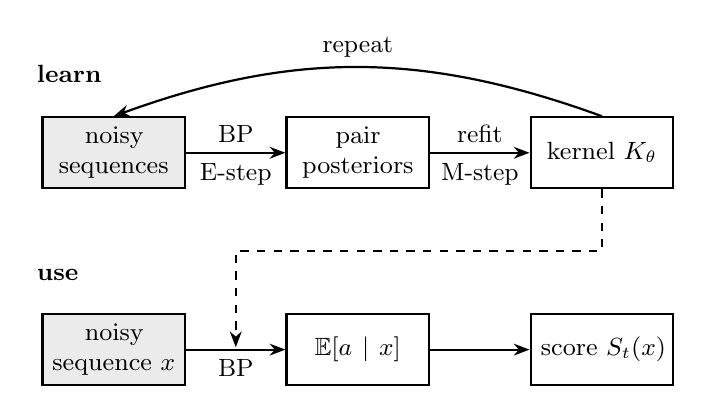
\begin{tikzpicture}[
    box/.style={draw,thick,align=center,font=\small,minimum height=9mm,inner sep=3pt,text width=1.6cm},
    data/.style={box,fill=black!8},
    arr/.style={-{Stealth[length=2mm]},thick},
    lab/.style={font=\small,align=center}]
  \node[font=\small\bfseries,anchor=west] at (-1.1,1.0) {learn};
  \node[data] (d) at (0,0) {noisy\\ sequences};
  \node[box] (p) at (3.1,0) {pair\\ posteriors};
  \node[box] (k) at (6.2,0) {kernel $K_\theta$};
  \draw[arr] (d) -- node[above,lab]{BP} node[below,lab]{E-step} (p);
  \draw[arr] (p) -- node[above,lab]{refit} node[below,lab]{M-step} (k);
  \draw[arr] (k.north) to[out=160,in=20] node[above,lab]{repeat} (d.north);
  \node[font=\small\bfseries,anchor=west] at (-1.1,-1.55) {use};
  \node[data] (x) at (0,-2.5) {noisy\\ sequence $x$};
  \node[box] (m) at (3.1,-2.5) {$\mathbb{E}[a\mid x]$};
  \node[box] (s) at (6.2,-2.5) {score $S_t(x)$};
  \draw[arr] (x) -- node[below,lab]{BP} (m);
  \draw[arr] (m) -- (s);
  \draw[thick,dashed,-{Stealth[length=2mm]}] (k.south) -- (6.2,-1.25) -| (1.55,-2.47);
\end{tikzpicture}

  \caption{\note{Learn: BP (E-step) gives pair posteriors, the refit (M-step) gives $K_\theta$, repeat. Use: BP with
  $K_\theta$ gives $\E[a\mid x]$, hence the score. Slide 11.}}
  \label{fig:em-loop}
\end{figure}

\note{J\'er\^ome (50:20): explain EM more, in the logic of the gradient of an expectation: BP gives the expectation;
the kernel is a controlled function of $\theta$; take the gradient of the expectation over $\theta$ and follow it, on a
given set of examples. E-step: pair posteriors $\xi_k(a,a')$, summed into expected counts $\Xi$. M-step: raise
$Q(\theta)=\iint\Xi\log K_\theta$. Fisher's identity: $\nabla Q=\nabla\log p_\theta(x)$ at $\theta_{\rm old}$, so the
likelihood never decreases (23:38).}

\note{Say explicitly (his worry at 39:37--41:27): there is NO backpropagation through BP. BP enters only through
$\Xi$, constant during the M-step; autograd only goes through $K_\theta$ and its grid normaliser
(\texttt{energy\_kernel.py}, E55). Also: the noise level is only in the E-step, so no noise schedule is needed to
learn the kernel.}

\subsection{Kernel families}
\label{sec:families}

\begin{figure*}[t]
  \centering
  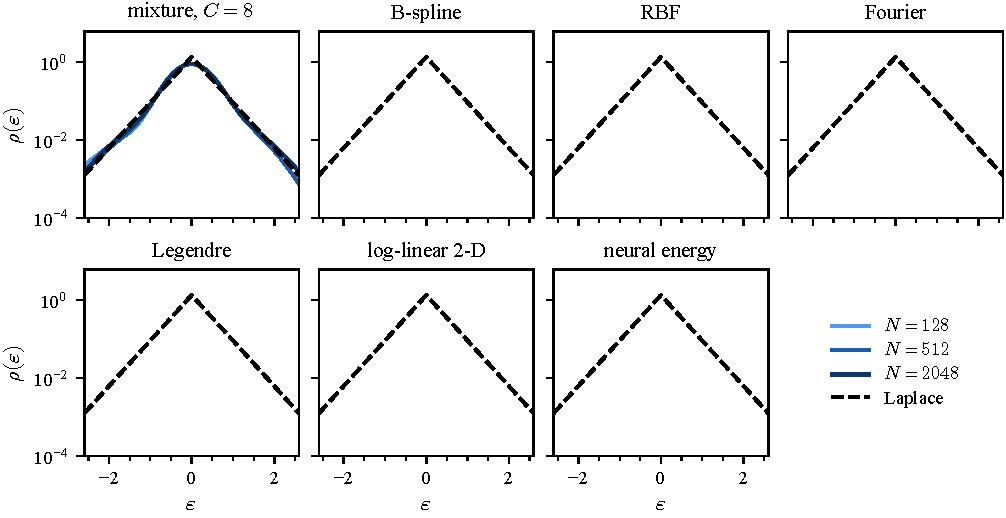
\includegraphics{fig_families}
  \caption{\note{Thesis Fig.~6.3 for every family (37:41): learned innovation law at $N=128$, $512$, $2048$ against
  the Laplace truth (dashed). Mixture from exp\_18; the other six from E56 (pending).}}
  \label{fig:families}
\end{figure*}

\note{J\'er\^ome (22:15, 26:41): why would the kernel be a mixture of $C$ Gaussians? Families he named: truncated
Fourier series (28:18), polynomials, Gaussian RBF, Mat\'ern (29:29). Put the series on $\log K$, not on $K$: positive
kernel, concave M-step. Local bases (spline, RBF) can make the kink; global (Fourier, Legendre) only by oscillating.
Shift families vs agnostic ones (log-linear 2-D, neural energy kernel: 2-layer MLP, 13:45, 39:37).}

\note{Mixture numbers (fig\_em\_innovation, App.~B): $\alpha$ within $0.1\%$ from $N=512$ ($2.4\%$ at $128$);
excess kurtosis only within $6$--$25\%$.}

\subsection{Against neural denoisers}
\label{sec:networks}

\begin{figure}[t]
  \centering
  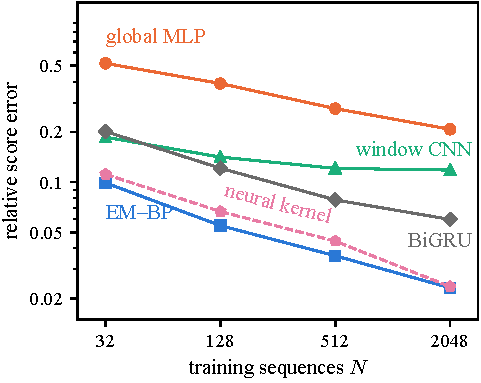
\includegraphics{fig_value_of_structure}
  \caption{\note{Slide 14 as one plot (21:25): EM--BP, global MLP, window CNN, and BiGRU (the best of six from
  $N=128$). Same test sequences, 16 seeds.}}
  \label{fig:value-of-structure}
\end{figure}

\begin{figure}[t]
  \centering
  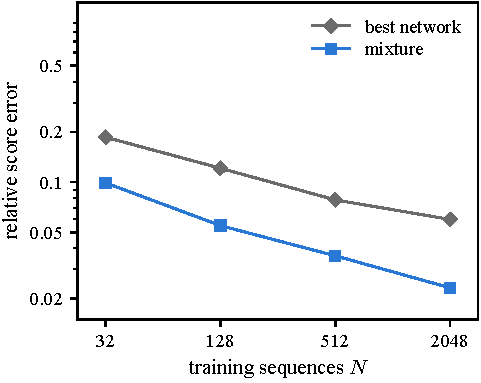
\includegraphics{fig_families_error}
  \caption{\note{Every kernel family against $N$, best network for reference. E56 (pending).}}
  \label{fig:families-error}
\end{figure}

\note{J\'er\^ome (21:25): this is where ML people will complain, so be careful. Networks: DSM on CLEAN sequences
(an advantage), screened on dev seeds, validation checkpoint; EM sees one noisy copy of each sequence.}

\note{Numbers (paired E02a/E03, mean per-seed ratio network/EM--BP, $N=32,128,512,2048$): MLP $5.79, 7.95, 7.88,
9.85$; window CNN $2.07, 2.87, 3.45, 5.58$; BiGRU $2.22, 2.45, 2.24, 2.83$. Honest headline: best network at each $N$,
$2.1$--$2.8\times$. EM--BP error $0.099\to0.023$; CNN $0.19\to0.12$ (flat: the window floor of Sec.~3). These replace
the thesis's $6.6$--$10.9\times$ and $2.3$--$6.1\times$.}

\subsection{Step efficiency}
\label{sec:steps}

\begin{figure*}[t]
  \centering
  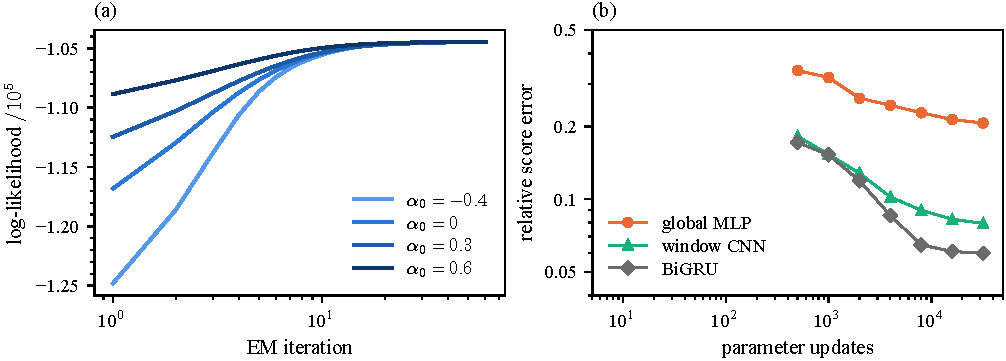
\includegraphics{fig_em_dynamics}
  \caption{\note{(a) EM log-likelihood against iteration, four starts. (b) Validation score error against parameter
  updates: EM iterations (E56, pending) and SGD steps (E03), $N=2048$.}}
  \label{fig:em-dynamics}
\end{figure*}

\note{J\'er\^ome (22:15, 23:50): dynamics curves; the claim is ``not only sample efficient, also step efficient''.
Wall-clock is less important (23:50). Careful: he expects $\sim10$ steps (25:16); measured: likelihood plateau in
$\sim20$ iterations, $\alpha$ settles in a median of 80 updates, the shape in 229 (tail 638) (thesis exp\_27). Still
2--3 orders fewer than the networks' $10^3$--$3\times10^4$ SGD steps. Per EM iteration: 3--6.6\,s at $N=2048$, one
CPU thread (E56 timing).}

\subsection{When the data are not Markov}
\label{sec:nonmarkov}

\begin{figure}[t]
  \centering
  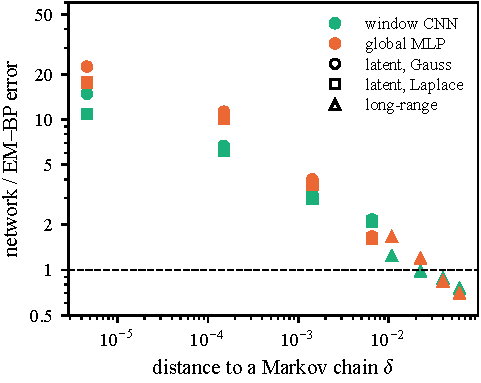
\includegraphics{fig_nonmarkov}
  \caption{\note{Network / EM--BP error against $\delta$, the distance per site to the closest first-order chain.
  Global latent (Gaussian and Laplace) and long-range couplings. Below 1 the network wins.}}
  \label{fig:nonmarkov}
\end{figure}

\note{J\'er\^ome (32:51--33:47): break the Markovianity and see how long it stays good, in the main text. Global latent
$a=(y+\beta g)/\sqrt{1+\beta^2}$; long-range $Q_{\rm AR}+\gamma Q_{\rm long}$. Numbers: at $\delta\approx5\times10^{-6}$
CNN $11$--$15\times$ worse, MLP $18$--$22\times$; break-even $\delta^\star\approx1$--$2\times10^{-2}$ (CNN),
$2$--$4\times10^{-2}$ (MLP); $\hat\alpha$ $0.848\to0.939$ at $\beta=1$. Second-order chain: not run yet.}

\section{Application: the stochastic Allen--Cahn field}
\label{sec:allen-cahn}

\begin{figure*}[t]
  \centering
  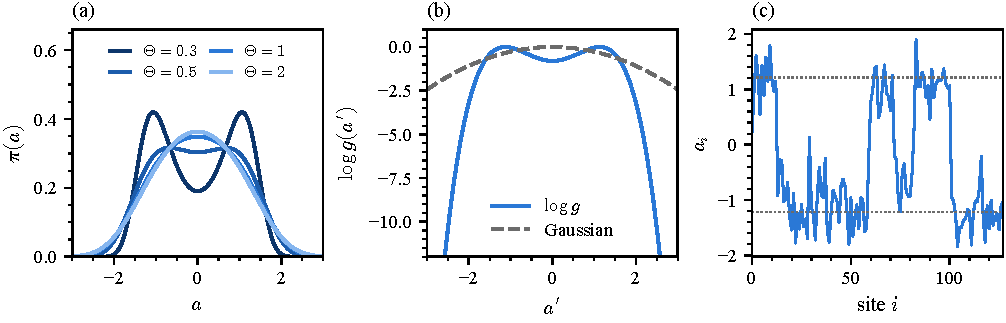
\includegraphics{fig_field}
  \caption{\note{(a) Single-site law at $\Theta=0.3$, $0.5$, $1$, $2$. (b) Kernel tilt $\log g$ against the Gaussian
  chain's quadratic. (c) One exact sample at $\Theta=0.3$; dotted: the wells.}}
  \label{fig:field}
\end{figure*}

\note{The application (12:01, 33:47). The SPDE $\partial_\tau\phi=\partial_x^2\phi-V'(\phi)+\sqrt{2\Theta}\eta$,
$V=\tfrac14(\phi^2-1)^2$; on a lattice its stationary law is a nearest-neighbour chain. Kernel = tilted walk
$\Normal(a';a,\gamma)g(a')$: the shape of the law of $a'$ depends on $a$. Cells: four $\Theta$, $L=32$, neighbour
correlation $0.85$ (E32).}

\begin{table}[t]
  \caption{\note{Error / best linear denoiser, $M=2048$, 16 seeds. Slide 15. Add the neural energy kernel row (E55).}}
  \label{tab:field}
  \centering
  \small
  \setlength{\tabcolsep}{4pt}
  \begin{tabular}{@{}lcccc@{}}
    \toprule
    $\Theta$ & 0.3 & 0.5 & 1 & 2\\
    \midrule
    site energy (5)          & 0.033 & 0.072 & 0.141 & 0.169\\
    tilted spline (25)       & 0.060 & 0.134 & 0.280 & 0.428\\
    log-linear 2-D (100)     & 0.184 & --    & 0.428 & --\\
    MDN (1{,}516)            & 0.228 & 0.422 & 0.738 & 0.838\\
    shift mixture (25)       & 1.004 & 1.004 & 1.014 & 1.021\\
    best network             & 0.484 & 1.174 & 2.157 & 3.044\\
    \bottomrule
  \end{tabular}
  % src: ~/Code/Thesis/jerome-call-2026-10-29-slide15.md (frozen E33 / E43 rows)
\end{table}

\note{J\'er\^ome's worry (38:50): at $\Theta=0.3$ the best network ($0.48$) beats the thesis kernel ($1.00$). Answer
from the frozen fits: the mixture is NOT collapsed (7.8 of 8 effective components); it is a shift family with linear
drift, so its best member is a Gaussian chain, and BP with it is linear. Every family whose law depends on $a$ beats
the best network in every cell, at $M=2048$ and $M=128$, including two with no field structure (log-linear 2-D $0.18$,
MDN $0.23$). Decide: keep the mixture row as the ``wrong family'' (as here) or drop it.}

\note{Data efficiency: with $M=128$ the site energy ($0.14$) beats the network with $2048$ ($0.48$). Parameter
recovery: $\hat\Theta/\Theta$ seed means $0.9995$--$1.0068$ (site energy, six cells, E33). Pending: E55, neural energy
kernel vs DDPM U-Net.}

\section{Discussion}
\label{sec:discussion}

\note{Half a column. The message in three sentences. Limits: first order (repair: pair state), one number per site
(vector state: $N_g^d$ grid), trees only (2-D lattices are loopy), grid cost $O(LN_g^2)$ and small $t$.}

\note{M\'ezard's defence questions: what happens with longer chains (BP linear in $L$, kernel independent of $L$; E03
length test); how this could improve how scores are computed for diffusion models (learn the local law, infer
globally; a hybrid with a network for what is not Markov).}

\paragraph{Related work.} \note{HMM / state-space EM, diffusion from corrupted data with EM, BP and hierarchical data
(J\'er\^ome's transformers paper), analytic denoisers. Keys already in references.bib:
\cite{baum1970,shumway1982em,cappe2005,daras2023ambient,rozet2024learning,bai2024em,garnierbrun2024transformers,kamb2024analytic,kadkhodaie2024generalization}.}


\section*{Impact statement}
\note{Required by ICML, not counted in the page limit. Two sentences.}

\bibliography{references}
\bibliographystyle{icml2026}

\newpage
\appendix
\onecolumn
\section{BP on a grid}
\label{app:bp}

\note{Grid, trapezoid weights, kernel matrix, the two sweeps, posterior mean, pair posteriors, log-likelihood from the
forward normalisers, cost.}

\label{app:numerics}
\begin{figure}[h]
  \centering
  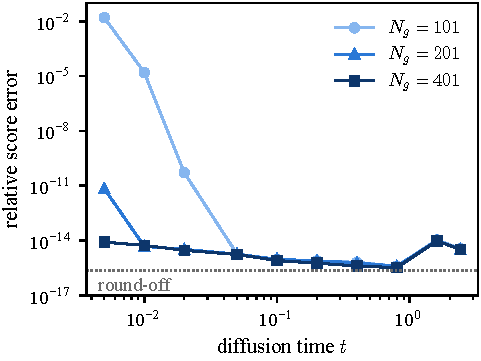
\includegraphics{fig_grid_gaussian}\hfill
  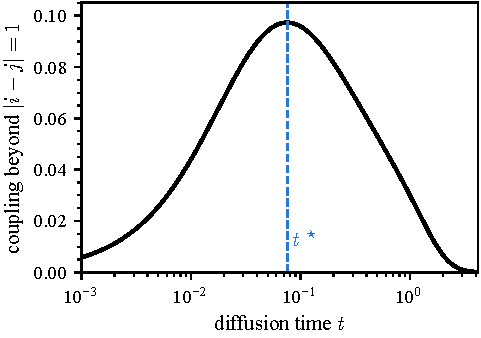
\includegraphics{fig_locality_curve}
  \caption{\note{Left: grid BP against $-Q_tx$, Gaussian chain, $N_g=101$, $201$, $401$ (round-off for
  $t\geq0.05$). Right: coupling of $Q_t$ beyond nearest neighbours against $t$, peak at $t^\star$.}}
  \label{fig:grid}
\end{figure}

\section{EM: M-steps}
\label{app:em}

\note{Closed forms (Gaussian and Laplace AR(1)), mixture ECM, log-linear (concave, observed minus expected), neural
(autograd on $Q$, GEM). Checkpoint ladder and selection.}

\begin{figure}[h]
  \centering
  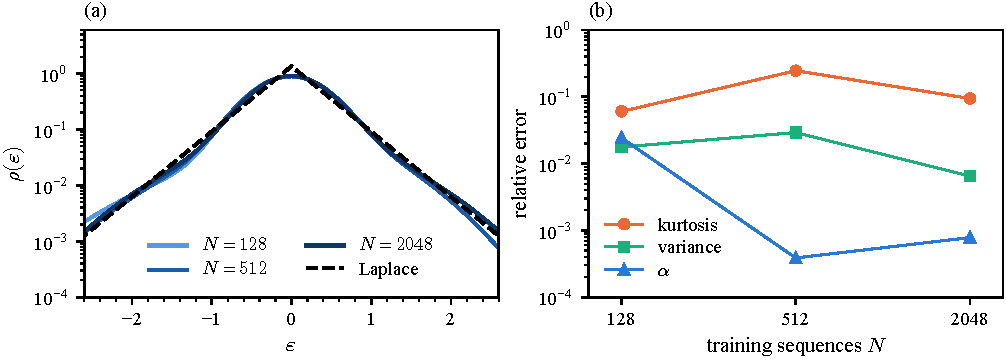
\includegraphics{fig_em_innovation}
  \caption{\note{Mixture ($C=8$): learned innovation law, and relative error of $\alpha$, variance and kurtosis
  against $N$ (thesis Fig.~6.3).}}
  \label{fig:em-innovation}
\end{figure}

\section{Sources of error}
\label{app:errors}

\note{J\'er\^ome (20:14): the error decomposition is ``typical appendix stuff''. Grid, misspecification, finite data,
EM stopping.}

\section{Network baselines}
\label{app:networks}

\note{Architectures and parameter counts (MLP 26{,}016, CNN 5{,}505, BiGRU 15{,}169), screen, recipe, pairing.}

\section{Allen--Cahn details}
\label{app:field}

\note{Cells, families, networks, the $M=128$ table (slide-15 note).}


\end{document}
